\chapter{Sequenzdiagramme}
Im Folgenden wird das Szenario \enquote{Event anlegen} ausführlich mit Pseudocode entwickelt, um eine Reihe an Sequenzdiagrammen zu erstellen, die den Sachverhalt visualisieren.

Bei der Darstellung der Sequenzdiagramme wurde auf die exakte Interaktion mit einer Datenbankschnittstelle oder CSV-Dateien verzichtet, da diese Details hier nicht von Relevanz sind. Stattdessen wird ein Datenbasisobjekt verwendet, welches abstrakt für alle Interaktionen des Datenschreibens und -lesens zuständig ist. Es wird auch angenommen, dass der Nutzer bereits eingeloggt ist und die entsprechende Benutzeroberfläche bereits geöffnet hat. Das setzen der grundlegenden Attribute von Objekten wird unter dem Begriff der \enquote{primitiven Attribute} zusammengefasst, wenn es möglich ist. Der Fokus liegt auf den Nachrichten und den Interaktionen dazwischen, weniger auf Details des Entwurfs.

\section{Szenariobetrachtung: Event anlegen}
In diesem Szenario wird von einem Organisator ein neues Event angelegt. Hierbei wird allerdings noch eine Vielzahl weiterer Objekte erzeugt, welche vom eigentlichen Eventobjekt referenziert werden. Hierzu zählen beispielsweise Bilder, Verweise oder Teileinheiten, welche ihrerseits wieder auf weitere Objekte verweisen können.

Das Szenario setzt sich aus mehreren Teilschritten zusammen: Zunächst muss ein initiales Eventobjekt erzeugt werden. Hierbei hat der Organisator die Möglichkeit, entweder mit einem leeren Eventobjekt zu starten oder aber ein Eventelement als Template für die Erstellung des Events zu verwenden. In diesem Fall würde das Event bereits mit einer Beschreibung, einer Kategorie und eventuell vordefinierten Teileinheiten sowie den zugehörigen Kostenschätzungen initialisiert. 

Im nächsten Schritt hat der Organisator die Möglichkeit, das Event mit Leben zu füllen, indem er ihm nach belieben Bilder, Verweise - beispielsweise auf beteiligte Firmen - sowie untergeordnete Teileinheiten zuweist und diese unter Umständen auch erstellt. Ferner weist er dem gesamten Event einen Start- und einen Endetermin sowie einen Verantwortlichen zu. Bei dem Verantwortlichen kann es sich sowohl um eine Einzelperson als auch eine Gruppe von Personen handeln.

Abschließend besteht für den Organisator noch die Möglichkeit, Änderungen an den primitiven Attributen des Events, also beispielsweise Name, Beschreibung oder Kategorie, vorzunehmen. Ist der Organisator mit dem Event zufrieden, kann es anschließend gesichert und damit seine Arbeit persistiert werden.

Aus Gründen der Übersichtlichkeit wurden die meisten der oben genannten Operationen, nämlich das Anlegen von Bildern, Verweisen und Teileinheiten sowie das Finden eines Verantwortlichen im Pseudo-Code in separate Funktionen ausgelagert und darum auch als separate Sequenzdiagramme modelliert, welche dann im Hauptdiagramm des Szenarios durch Interaktionsreferenzen aufgerufen werden. 

\section{Pseudo-Code}
Um Übersichtlichkeit und klare Struktur zu ermöglichen, wurde der Pseudocode in kleinere Unterprogramme geteilt, die aufgerufen werden. Dieses ermöglicht es ebenfalls, Abläufe nicht redundant darzustellen.

Der Kunde ist Auftraggeber und hat Wissen über die gewünschten Details des Events. Der Organisator ist Nutzer des Systems und plant die konkreten Details des Events.

\lstinputlisting[style=Pseudocode, firstline=3, lastline=43, caption={Szenario Event anlegen}]{Quellcode/sequence_diagram_pseudo.txt}

Deutlich zu erkennen sind die vielen Aufrufe zu Unterprogrammmen für das Anlegen und Hinzufügen der verschiedenen Objekte, die das Event ausmachen.

\lstinputlisting[style=Pseudocode, firstline=45, lastline=98, caption={Szenario Teileinheit anlegen}]{Quellcode/sequence_diagram_pseudo.txt}

Hier ist deutlich die Ähnlichkeit zu \code{EVENT-ANLEGEN} zu sehen. Besonders ist jedoch der rekursive Aufruf auf sich selbst, der es ermöglicht, einen Baum an Teileinheiten aufzubauen. Auch zu beachten ist, dass einer Teileinheit entweder Hilfsmittel oder Teileinheiten hinzugefügt werden können. Es ist nicht möglich, beides hinzuzufügen.

\lstinputlisting[style=Pseudocode, firstline=100, lastline=122, caption={Szenario Verantwortlichen finden}]{Quellcode/sequence_diagram_pseudo.txt}

Als Verantwortlicher kann eine Gruppe oder eine Einzelperson gewählt werden, dadurch sind die zwei verschiedenen Ausführungspfade vorhanden.

\lstinputlisting[style=Pseudocode, firstline=124, lastline=135, caption={Szenario Mitarbeiter finden}]{Quellcode/sequence_diagram_pseudo.txt}

Beim Finden eines Mitarbeiters für die Verantwortlichkeit werden nur die zu der Zeit verfügbaren Mitarbeiter angezeigt. Solange der Organisator die Suchkriterien dabei ändert, wird die Liste immer wieder aktualisiert. Wenn der Organisator sich für einen Mitarbeiter aus der Liste entscheiden sollte, wird dieser zurückgegeben. Stattdessen gibt es noch die Möglichkeit, dass der Organisator einen neuen Mitarbeiter anlegen möchte, da dieser bisher nicht im System erfasst ist. Dann wird das Unterprogramm \code{MITARBEITER-ANLEGEN} aufgerufen.

\lstinputlisting[style=Pseudocode, firstline=137, lastline=162, caption={Szenario Verweis anlegen}]{Quellcode/sequence_diagram_pseudo.txt}

Beim Anlegen eines Verweises sind alle Attribute optional. Dieses ist deutlich dadurch zu sehen, dass das Hinzufügen immer an die Bedingung geknüpft ist, dass dieses vom Nutzer gewünscht ist.

\lstinputlisting[style=Pseudocode, firstline=164, lastline=172, caption={Szenario Bild anlegen}]{Quellcode/sequence_diagram_pseudo.txt}

Hier ist deutlich zu sehen, dass in einem Bildobjekt keine Bilddaten gespeichert werden. Stattdessen ist in dem Objekt bloß der Dateiname der entsprechenden Datei im zentralen Verzeichnis hinterlegt. Auch interessant ist, dass zum Verhindern von Namensdopplungen in einer Schleife ein einzigartiger Name gesucht wird.

\lstinputlisting[style=Pseudocode, firstline=174, lastline=189, caption={Szenario Ansprechperson anlegen}]{Quellcode/sequence_diagram_pseudo.txt}

Beim Anlegen einer Ansprechperson handelt es sich um einen recht einfachen Vorgang ohne besondere Logik, da ein Ansprechpersonenobjekt nur aus seinen primitiven Attributen sowie den Kontaktdaten besteht, welche in einem separaten Unterprogramm festgelegt werden.

\lstinputlisting[style=Pseudocode, firstline=191, lastline=214, caption={Szenario Verwendung anlegen}]{Quellcode/sequence_diagram_pseudo.txt}

Um ein Hilfsmittel für eine Teileinheit zu buchen, wird das Koordinatorobjekt \enquote{Verwendung} erstellt. Diese Verwendung speichert Informationen über die Relation zwischen Teileinheit und Hilfsmittel.

\lstinputlisting[style=Pseudocode, firstline=216, lastline=239, caption={Szenario Hilfsmittel anlegen}]{Quellcode/sequence_diagram_pseudo.txt}

Beim Anlegen eines Hilfsmittels ist die Unterscheidung zwischen Gebrauchs- und Verbrauchsgut zu beachten. Zum einen muss der Organisator bei einem Gebrauchsgut die vorhandene Gesamtzahl angeben, während bei einem Verbrauchsgut die aktuell verfügbare Menge einzutragen ist. Ferner wird bei der Erstellung eines Verbrauchsgutes auch ein Verweis angelegt, da zu jedem Verbrauchsgut ein Verweis auf den Lieferanten des jeweiligen Hilfsmittels gehört.

\lstinputlisting[style=Pseudocode, firstline=241, lastline=274, caption={Szenario Mitarbeiter anlegen}]{Quellcode/sequence_diagram_pseudo.txt}

Wie man sieht, werden beim Anlegen eines Mitarbeiters nicht nur die primitiven Attribute des Mitarbeiters und dessen Kontaktdaten gepflegt, sondern auch die ihm zugewiesenen Rollen vergeben. Das Hinzufügen weiterer Rollen ist natürlich nur möglich, solange der Mitarbeiter noch nicht alle im System verfügbaren Rollen besitzt. Anschließend werden dem Mitarbeiter ein oder mehrere Beschäftigungszeiträume zugewiesen. Auch bei diesen wird stets überprüft, ob Start- und Endetermin plausibel sind.

\section{Diagramme}

In den Diagrammen werden Interaktionsreferenzen verwendet, um sich auf Unterdiagramme mit Verfeinerungen zu beziehen. In den verfeinerten Diagrammen taucht das Objekt \enquote{Observer} auf, welches jeweils den aufrufenden View darstellen soll. Es wurde sich für diese Umsetzung in den Diagrammen entschieden, da das gleiche Diagramm von verschiedenen Diagrammen aus referenziert werden kann. Ein Beispiel dafür ist das Diagramm \enquote{Teileinheit anlegen}, welches von \enquote{Teileinheit anlegen} und \enquote{Event anlegen} referenziert wird. Je nachdem, wird die angelegte Teileinheit der \enquote{TeileinheitGUI} oder \enquote{EventGUI} zurückgegeben, aber im Diagramm wird dafür einfach der \enquote{Observer} als abstrakte Darstellung verwendet.

\subsection{Event anlegen}

\begin{figure}[ht!]
    \centering
    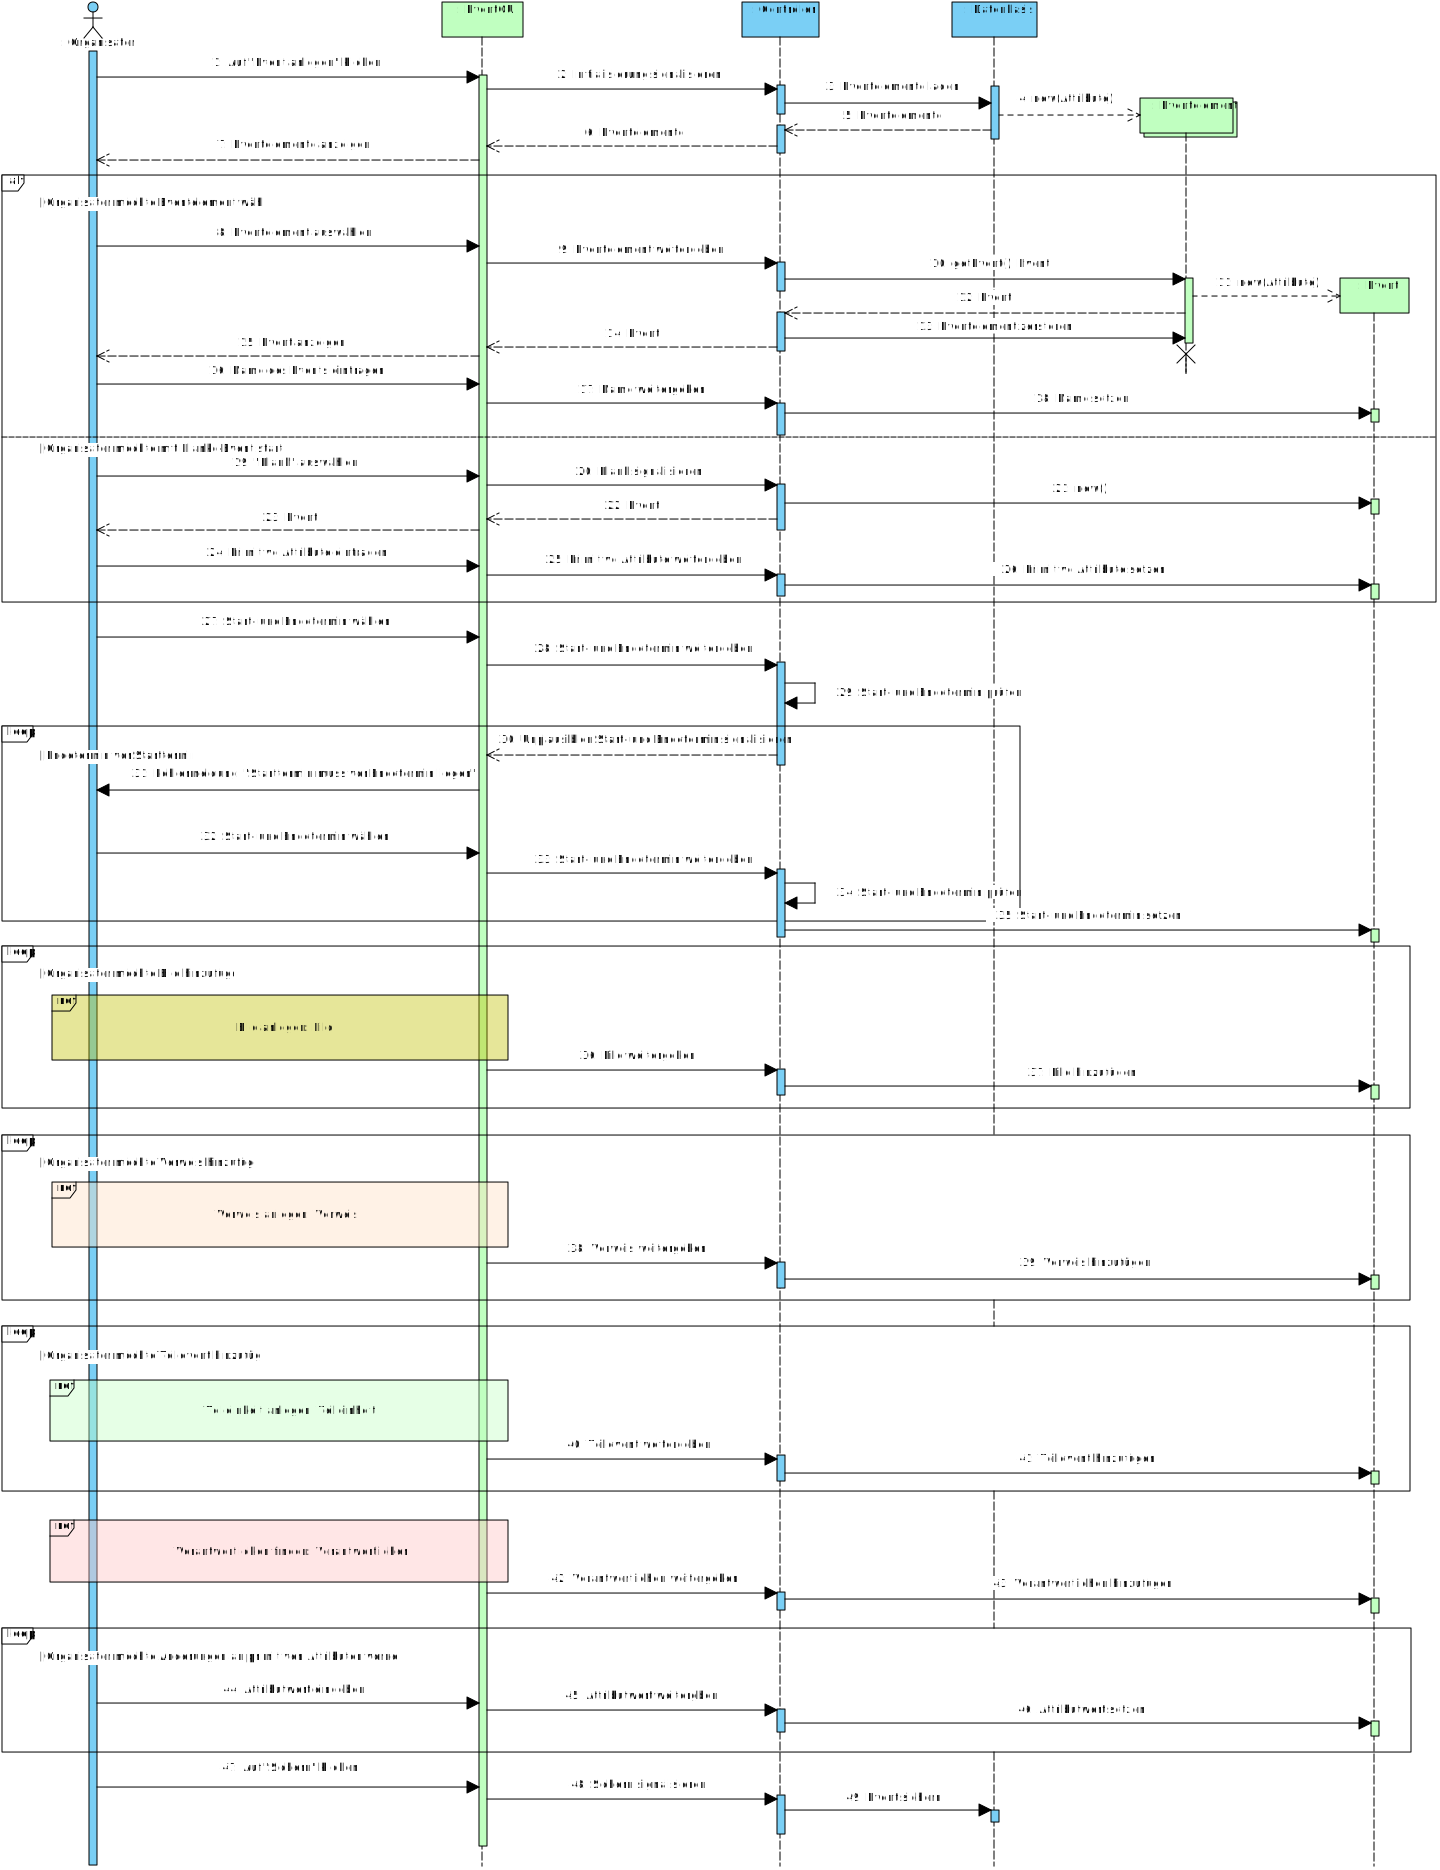
\includegraphics[width=0.98\columnwidth]{Bilder/seq_Event_anlegen.pdf}
    \caption{Szenario Event anlegen}
    \label{seq:event-anlegen}
\end{figure}

Das in \autoref{seq:event-anlegen} modellierte Szenario \enquote{Event anlegen} wird dadurch begonnen, dass der Organisator sich entschließt ein Event anzulegen und dieses dem System mitteilt. Zu Beginn muss entschieden werden, ob ein Eventelement als Vorlage verwendet werden soll oder mit einem leeren Event gestartet wird. Dafür werden zuerst alle verfügbaren Eventelemente aus der Datenbasis geladen und dem Nutzer angezeigt.

Möchte der Organisator mit einem Eventelement als Vorlage starten, so wählt er eine dieser Optionen und es beginnt der Prozess, aus dieser Vorlage ein Event zu erstellen. Jegliche primitiven Attribute des Eventelementes sowie alle dem Eventelement zugewiesenen Objekte werden dem neuen Event bei der Erschaffung direkt zugewiesen. Lediglich der Name muss durch den Nutzer noch manuell gesetzt werden, um zu vermeiden, dass sehr viele Events mit dem Namen des Eventelementes erstellt werden, denn generische Namen helfen dem Nutzer nicht, das Event von anderen zu unterscheiden.

Möchte der Organisator stattdessen mit einem leeren Eventobjekt starten, so wird zuerst ein leeres Eventobjekt erstellt, welches vom Organisator manuell mit primitiven Attributen befüllt werden muss. In beiden Fällen ist jetzt ein Eventobjekt vorhanden, welches vollständig befüllte primitive Attribute besitzt.

Anschließend werden Start- und Endetermin des Events vom Organisator eingetragen. Sollte der Endetermin vor dem Starttermin liegen, wird der Nutzer mit einer Fehlermeldung darüber unterrichtet. Diese Bedingung wird in einer Schleife wiederholt geprüft, bis der Fehler korrigiert wurde. Abschließend können dieser Start- und Endetermin gesetzt werden.

Das Hinzufügen der Objekte Teileinheit, Verweis und Bild ist hier auf gleiche Weise dargestellt. Es wird jeweils solange in einer Schleife verweilt, bis alle Objekte des gleichen Typs angelegt wurden. In der Schleife wird durch eine Interaktionsreferenz gezeigt, dass auf ein Unterprogramm verwiesen wird. Diese sind jeweils in den weiteren Diagrammen verfeinert dargestellt. Das Unterprogramm gibt jeweils ein Objekt des entsprechenden Typs zurück, welches dann zum Eventobjekt hinzugefügt wird.

Nachdem dieses getan ist, wird noch der Verantwortliche gesetzt. Dafür wird in einem Unterprogramm der Verantwortliche gefunden und anschließend hier nur noch als solcher im Eventobjekt gesetzt.

Zum Schluss kann der Organisator noch Änderungen an Attributen des Eventobjektes vornehmen, solange dieses nötig ist. Diese werden jeweils auf dem Eventobjekt gesetzt. Ist der Organisator vorerst fertig mit dem Bearbeiten des Events, so bestätigt er die Sicherung des Events. Dieses führt dazu, dass das Event auf der Datenbasis gesichert und damit persistent gespeichert wird.

\FloatBarrier

\subsection{Teileinheit anlegen}

\begin{figure}[ht!]
    \centering
    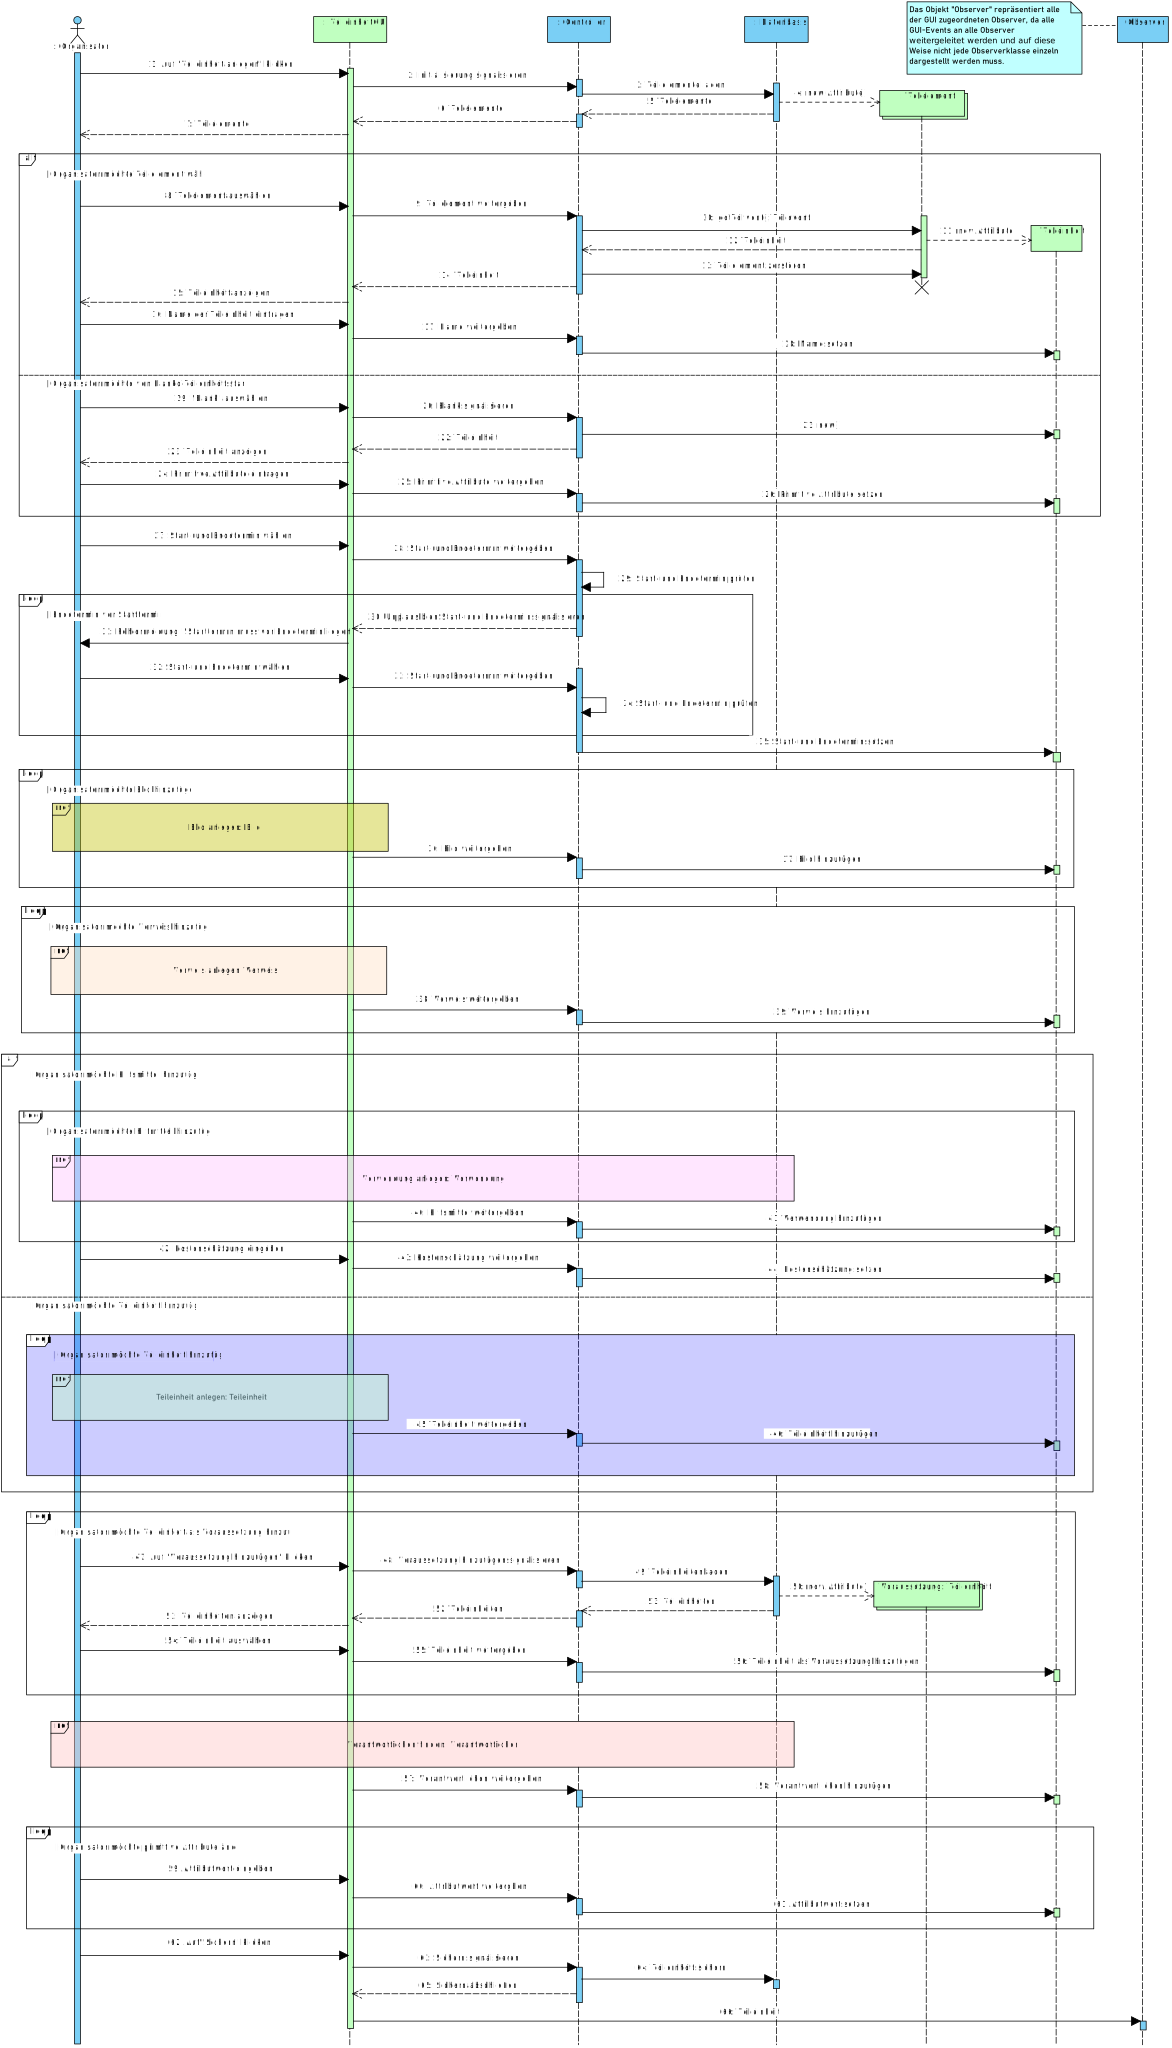
\includegraphics[width=0.7\columnwidth]{Bilder/seq_Teilevent_anlegen.pdf}
    \caption{Szenario Teileinheit anlegen}
    \label{seq:teileinheit-anlegen}
\end{figure}

Das Anlegen einer Teileinheit wurde in \autoref{seq:teileinheit-anlegen} modelliert. Hier klickt der Organisator zunächst auf \enquote{Teileinheit anlegen}, anschließend werden alle verfügbaren Teilelemente geladen und dem Organisator angezeigt. Nun hat der Organisator folgende mittels eines alt-Fragments modellierte Möglichkeiten: Im ersten Fall kann er die neue Teileinheit auf Basis eines der angezeigten Teilelemente erstellen, indem er dieses auswählt. In diesem Fall wird dann ein Teileinheitobjekt auf dem Teilelement generiert, anschließend werden die beim Laden erzeugten Teilelementobjekt zerstört. Nun muss der Organisator nur noch den Namen der Teileinheit eintragen, dann wird ihm die neue Teileinheit angezeigt. Im zweiten Fall, bei dem der Organisator kein Teilelement auswählt, wird mittels eines Konstruktoraufrufs eine leere Teileinheit erzeugt und dem Organisator angezeigt, sodass er die Möglichkeit hat, die primitiven Attribute der Teileinheit zu befüllen, welche anschließend im Teileinheitobjekt gesetzt werden.

Die folgenden Schritte sind nun wieder für beide der oben beschriebenen Pfade identisch. Zunächst wählt der Organisator einen Start- und einen Endetermin. Liegt der Starttermin vor dem Endetermin wird ihm eine Fehlermeldung angezeigt und er wird aufgefordert, einen neuen Start- und Endetermin auszuwählen. Dieser Vorgang wiederholt sich solange, bis der Starttermin vor dem Endetermin liegt, daher wurde diese Aktion als loop-Fragment modelliert.

Als nächstes hat der Organisator die Möglichkeit, der Teileinheit Bilder und Verweise hinzuzufügen. Hierzu müssen die Bild- und Verweisobjekte jedoch erst angelegt werden. Diese beiden Szenarien wurden allerdings in separaten Sequenzdiagrammen modelliert, welche hier mit Hilfe von Interaktionsreferenzen aufgerufen werden. Da der Organisator einer Teileinheit Bilder und Verweise in beliebiger Anzahl hinzufügen kann, finden das Anlegen und hinzufügen der Verweis- und Bildobjekte jeweils innerhalb eines loop-Fragmentes statt.

Im nächsten Schritt muss der Organisator wählen: Er kann der Teileinheit entweder weitere untergeordnete Teileinheiten hinzufügen oder er kann der Teileinheit Hilfsmittel hinzufügen. Diese beiden Möglichkeiten wurden durch ein alt-Fragment modelliert. Möchte der Organisator Hilfsmittel hinzufügen, so wird das Sequenzdiagramm \enquote{Verwendung anlegen} mittels einer Interaktionsreferenz aufgerufen und die entstandene Verwendung der Teileinheit hinzugefügt. Wie auch bei den Bildern und Verweisen, können einer Teileinheit beliebig viele Hilfsmittel hinzugefügt werden, daher befindet sich auch dieser Vorgang in einem loop-Fragment. Entscheidet sich der Organisator für das Hinzufügen weiterer Teileinheiten, müssen auch diese zuerst angelegt werden. Dies geschieht mittels eines rekursiven Aufrufs des hier beschrieben Sequenzdiagramms \enquote{Teileinheit anlegen}. Nun kann die erstellte Teileinheit der aktuellen hinzugefügt werden. Da jede Teileinheit beliebig viele Teileinheiten besitzen kann, befinden sich auch diese beiden Vorgänge innerhalb eines loop-Fragments.

Da Teileinheiten auch von einander abhängig sein können, hat der Organisator nun die Möglichkeit, vorhandene Teileinheiten als Voraussetzung für die aktuelle hinzuzufügen. Hierzu klickt er auf \enquote{Teileinheit als Voraussetzung hinzufügen}. Anschließend werden die vorhandenen Teileinheiten aus der Datenbasis geladen und angezeigt, sodass er die Möglichkeit hat, die gewünschte Teileinheit auszuwählen, welche der aktuellen dann als Voraussetzung hinzugefügt wird. Auch dieser Vorgang kann sich beliebig oft wiederholen und befindet sich darum in einem loop-Fragment.

Als nächstes muss ein Verantwortlicher für die Teileinheit gefunden werden. Dies geschieht mittels einer Interaktionsreferenz auf das Sequenzdiagramm \enquote{Verantwortlichen finden}. Der gefundene Verantwortliche, bei dem es sich sowohl um einen einzelnen Mitarbeiter, als auch um eine Gruppe von Mitarbeiter handeln kann, wird der Teileinheit als Verantwortlicher hinzugefügt.

Zuletzt hat der Organisator noch einmal die Möglichkeit, die primitiven Attribute der Teileinheit zu ändern. Dies kann beliebig oft geschehen und findet darum in einem loop-Fragment statt. Hierzu gibt der Organisator den neuen Attributwert ein, welcher anschließend in der Teileinheit gesetzt wird.
Abschließend klickt der Organisator auf \enquote{sichern}, sodass diese in der Datenbasis gespeichert wird.

\FloatBarrier

\subsection{Verantwortlichen finden}

\begin{figure}[ht!]
    \centering
    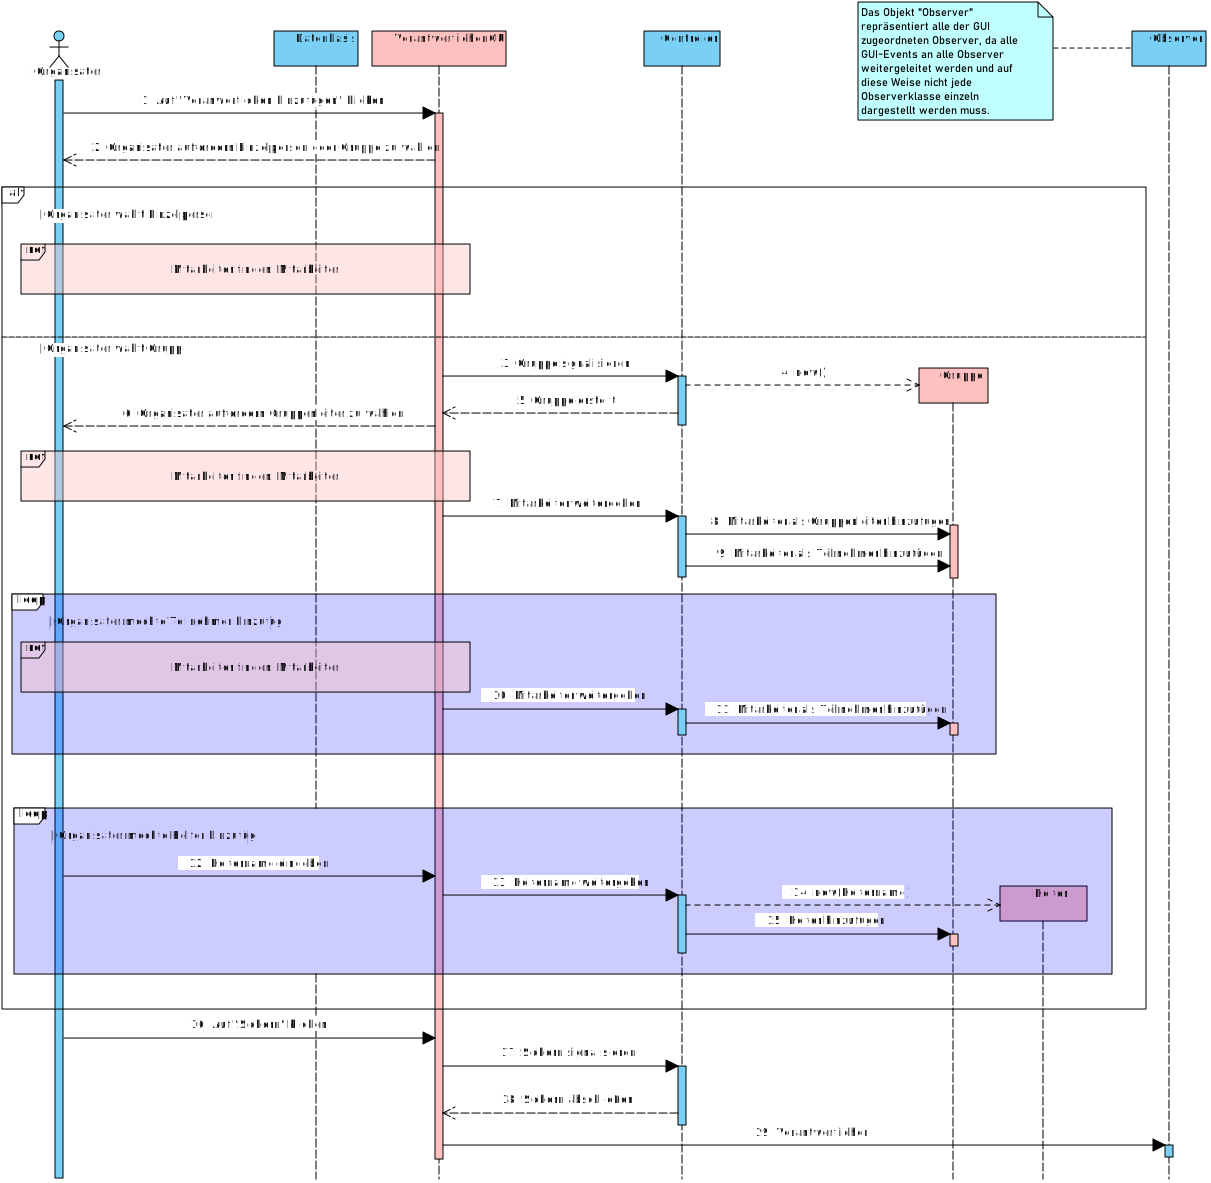
\includegraphics[width=0.98\columnwidth]{Bilder/seq_Verantwortlichen_finden.pdf}
    \caption{Szenario Verantwortlichen finden}
    \label{seq:verantwortlichen-finden}
\end{figure}

Beim Finden eines Verantwortlichen, was in \autoref{seq:verantwortlichen-finden} modelliert wurde, wird der Organisator zunächst aufgefordert, zu wählen, ob es sich bei dem Verantwortlichen um eine Gruppe oder eine Einzelperson handeln soll. Von hier an gibt es zwei mögliche Pfade: Entscheidet sich der Organisator für eine Einzelperson, so wird das Sequenzdiagramm \enquote{Mitarbeiter finden} mittels einer Interaktionsreferenz aufgerufen. Im zweiten Fall, wenn der Organisator sich für eine Gruppe als Verantwortlichen entscheidet, wird zunächst ein neues Gruppenobjekt erzeugt und der Organisator aufgefordert, einen Gruppenleiter zu bestimmen. Auch dies geschieht mit Hilfe des Sequenzdiagramms \enquote{Mitarbeiter finden}. Der so gefundene Mitarbeiter wird dem Gruppenobjekt dann sowohl als Gruppenleiter als auch als Teilnehmer hinzugefügt. Nun können der Gruppe noch beliebig viele weitere Teilnehmer hinzugefügt werden. Darum finden die beiden folgenden Schritte in einem loop-Fragment statt: Zunächst wird das Sequenzdiagramm \enquote{Mitarbeiter hinzufügen} aufgerufen. Der gefundene Mitarbeiter wird dann dem Gruppenobjekt als Teilnehmer hinzugefügt. Zuletzt hat der Organisator noch die Möglichkeit der Gruppe externe Helfer hinzuzufügen. Hierzu muss der Organisator lediglich den Namen des Helfers eingeben, anschließend wird eines neues Helferobjekt erzeugt, welches dann dem Gruppenobjekt hinzugefügt wird. Da in einer Gruppe auch beliebig viele Helfer sein können, findet auch dieser Vorgang innerhalb eines loop-Fragments statt. 

\FloatBarrier

\subsection{Mitarbeiter finden}

\begin{figure}[ht!]
    \centering
    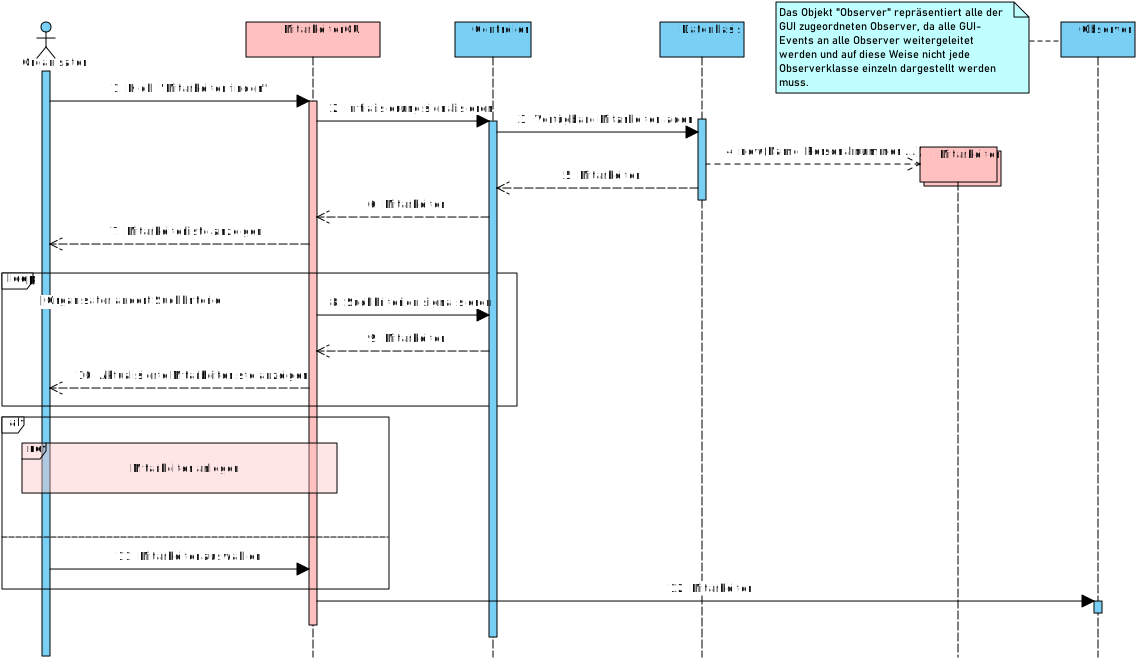
\includegraphics[width=0.98\columnwidth]{Bilder/seq_Mitarbeiter_finden.pdf}
    \caption{Szenario Mitarbeiter finden}
    \label{seq:mitarbeiter-finden}
\end{figure}

Um einen Mitarbeiter zu finden, klickt der Organisator zunächst auf \enquote{Mitarbeiter finden} wie man in \autoref{seq:mitarbeiter-finden} erkennen kann. Anschließend werden alle zwischen Start- und Endetermin verfügbaren Mitarbeiter aus der Datenbasis geladen und dem Organisator angezeigt. Nun kann der Organisator die verfügbaren Mitarbeiter nach ihren Attributen filtern. Hierzu ändert er die Suchkriterien, dann wird ihm eine aktualisierte Liste der Mitarbeiter angezeigt. Dieser Vorgang wiederholt sich, so oft der Organisator die Suchkriterien ändert, weshalb sich dieser in einem loop-Fragment befindet.

Nun gibt es zwei Möglichkeiten: Hat der Organisator einen passenden Mitarbeiter gefunden, wählt er diesen aus. Findet er keinen passenden Mitarbeiter, kann ein neuer angelegt werden und das Sequenzdiagramm \enquote{Mitarbeiter anlegen} wird aufgerufen.

\FloatBarrier
\newpage

\subsection{Verweis anlegen}

\begin{figure}[ht!]
    \centering
    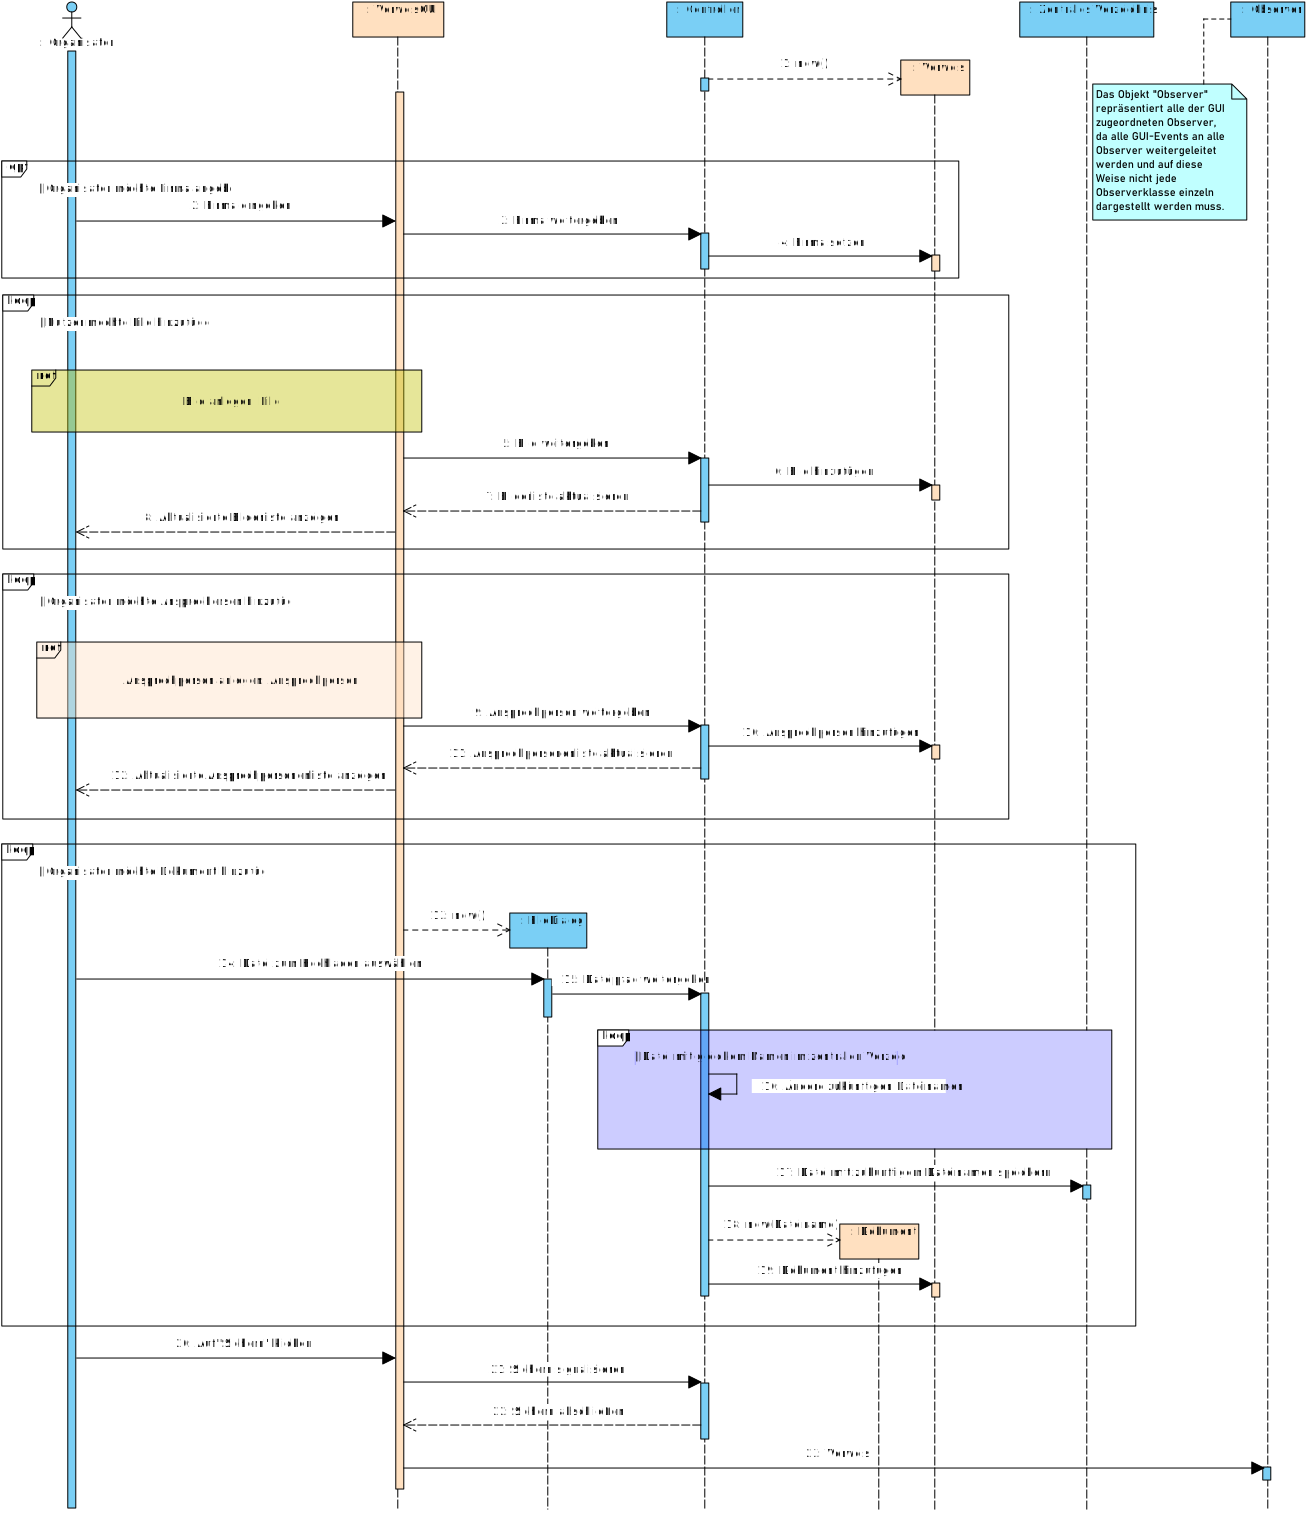
\includegraphics[width=0.98\columnwidth]{Bilder/seq_Verweis_anlegen.pdf}
    \caption{Szenario Verweis anlegen}
    \label{seq:verweis-anlegen}
\end{figure}

\FloatBarrier

Das Szenario \enquote{Verweis anlegen} ist in \autoref{seq:verweis-anlegen} dargestellt. Besonders am Verweisobjekt ist, dass jegliche seiner Attribute optional sind und es nicht alleine vorhanden sein kann. Daher wird das Objekt nicht zum Ende selbst in der Datenbasis, sondern nur als Teil des Events gesichert.

Zu Beginn des Szenarios wird ein vollständig leeres Verweisobjekt angelegt. Es besteht die Option, eine Firma anzugeben, zu der dieser Verweis gehört. Dieses primitive Attribut wird dann gesetzt.

Anschließend können in drei Schleifen die referenzierten Objekte Bild, Ansprechperson und Dokument angelegt und zum Verweis hinzugefügt werden. Das Bild und die Ansprechperson werden jeweils in anderen Unterprogrammen angelegt und hier dann nur noch zum Verweis hinzugefügt.

Da keine andere Entität Dokumente beinhalten kann, wurde sich dafür entschieden, das Anlegen eines Dokumentes nicht auf ein weiteres Unterprogramm auszulagern, sondern direkt hier zu beschreiben. Dazu wird vom Organisator eine Datei zum Hochladen ausgewählt. Es wird geprüft, ob im zentralen Verzeichnis bereits eine Datei mit dem gleichen Namen existiert. Sollte das der Fall sein, so wird der Name der Datei angepasst. Dieses wird in einer Schleife wiederholt, bis ein einzigartiger Name gefunden wurde. Dadurch wird garantiert, dass keine vorhandene Datei überschrieben wird. Wurde ein Name gefunden, so wird die Datei im zentralen Verzeichnis mit dem entsprechenden Namen abgelegt und ein Dokumentobjekt mit der Referenz auf diese Datei angelegt. Dieses Dokumentobjekt wird abschließend dem Verweis hinzugefügt.

\FloatBarrier
\newpage

\subsection{Bild anlegen}

\begin{figure}[ht!]
    \centering
    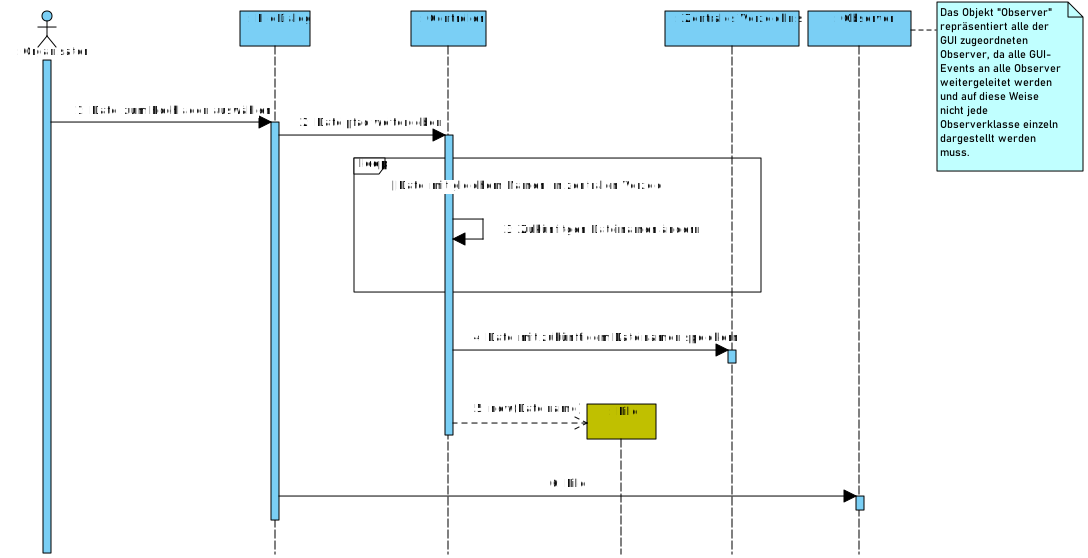
\includegraphics[width=0.98\columnwidth]{Bilder/seq_Bild_anlegen.pdf}
    \caption{Szenario Bild anlegen}
    \label{seq:bild-anlegen}
\end{figure}

In \autoref{seq:bild-anlegen} ist das Anlegen eines Bildes dargestellt. Dieses verläuft analog zu dem Prozess, ein Dokument anzulegen. Es wird ebenfalls eine Datei zum Hochladen gewählt, ein einzigartiger Name gefunden und anschließend die Datei im zentralen Verzeichnis abgelegt. Abschließend wird ein Bildobjekt mit Referenz auf die neu erstellte Datei erzeugt.

\FloatBarrier

\subsection{Ansprechperson anlegen}

In \autoref{seq:ansprechperson-anlegen} ist das Anlegen einer Ansprechperson dargestellt. Es werden zuerst die primitiven Attribute gesetzt und anschließend ein Kontaktdatenobjekt angelegt und dieses als Kontaktdaten der Ansprechperson gesetzt. Da die Telefonnummer ein verpflichtendes Attribut der Kontaktdaten ist, wird diese zu Beginn direkt vom Organisator eingegeben. Anschließend gibt es die Möglichkeit, die E-Mail-Adresse und die Anschrift anzugeben. Diese Möglichkeiten werden jeweils durch einen opt-Frame dargestellt. Zum Schluss wird das Kontaktdatenobjekt mit allen zuvor eingegebenen Daten erstellt.

\begin{figure}[ht!]
    \centering
    \includegraphics[width=0.98\columnwidth]{Bilder/seq_Ansprechperson_anlegen.pdf}
    \caption{Szenario Ansprechperson anlegen}
    \label{seq:ansprechperson-anlegen}
\end{figure}

\FloatBarrier

\subsection{Verwendung anlegen}

\begin{figure}[ht!]
    \centering
    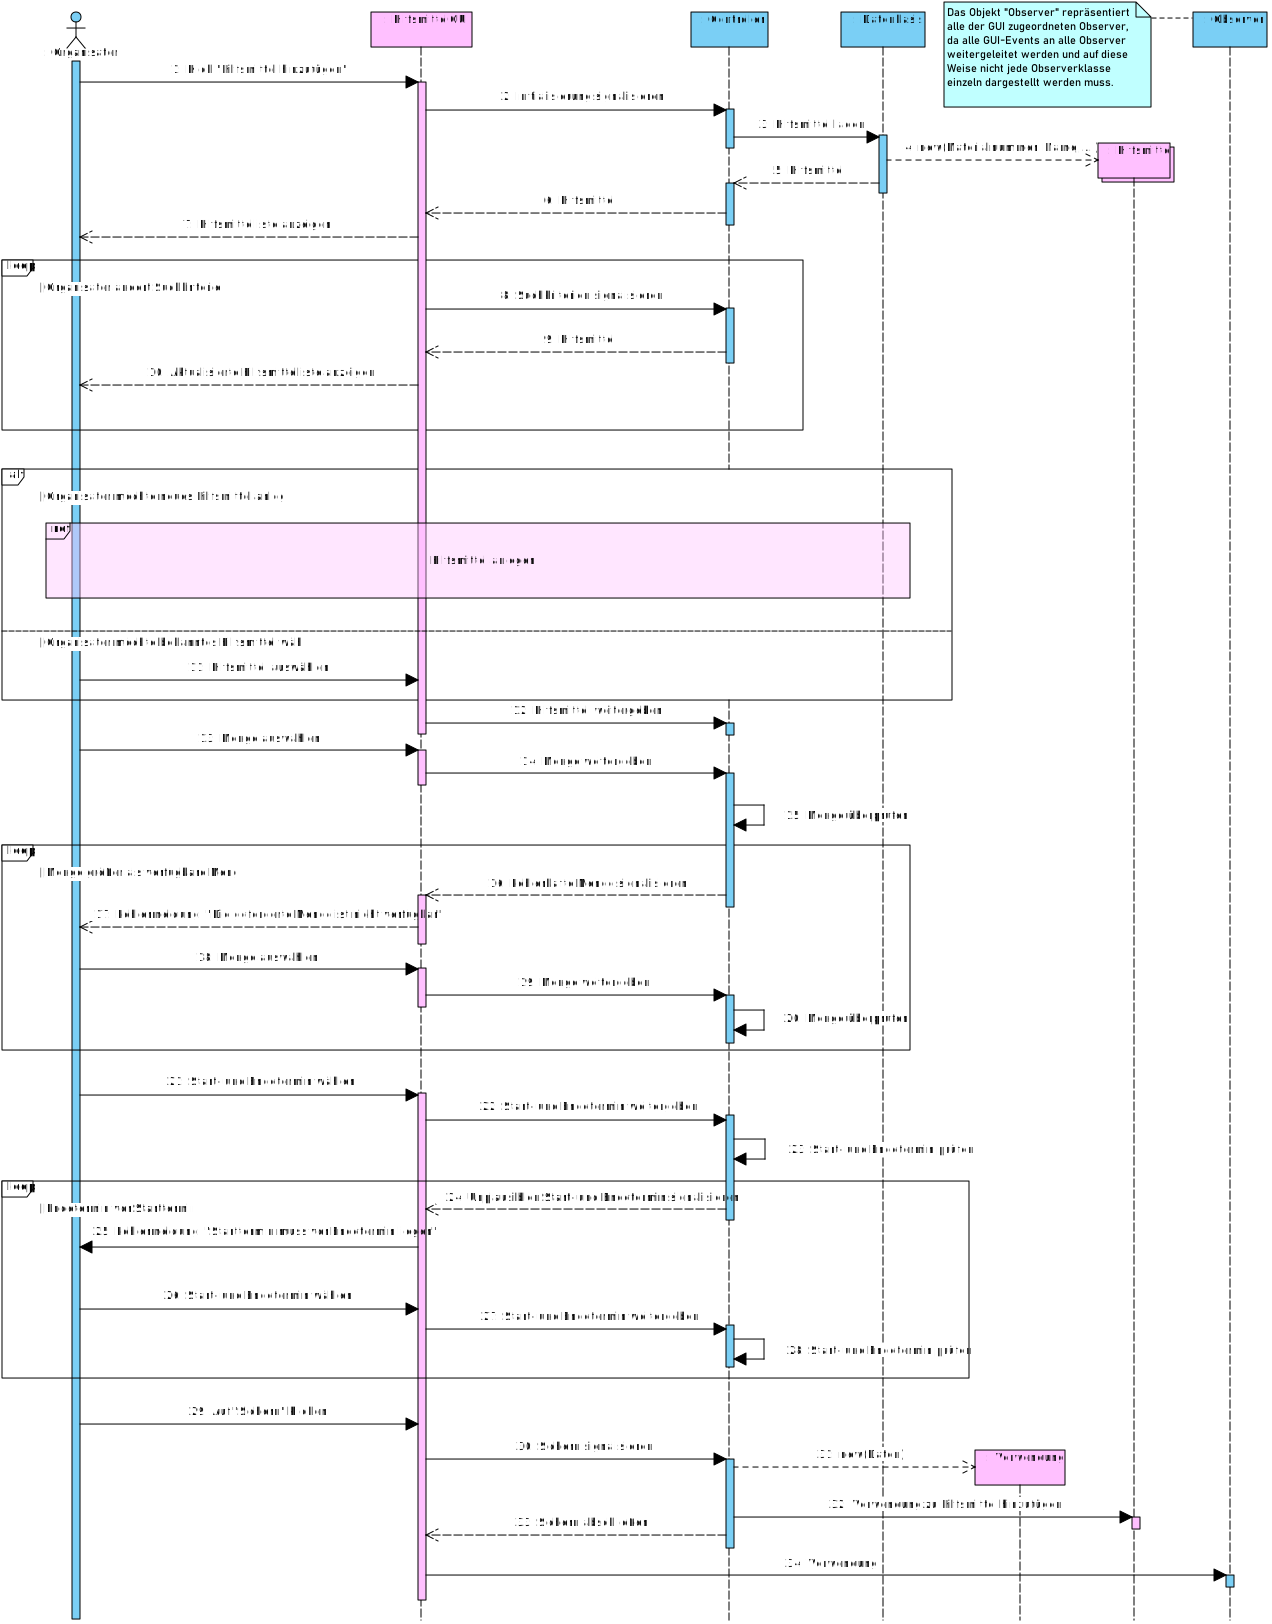
\includegraphics[width=0.9\columnwidth]{Bilder/seq_Verwendung_anlegen.pdf}
    \caption{Szenario Verwendung anlegen}
    \label{seq:verwendung-anlegen}
\end{figure}

Beim Anlegen einer Verwendung werden, wie in \autoref{seq:verwendung-anlegen} gezeigt, zunächst alle verfügbaren Hilfsmittel aus der Datenbasis geladen und dem Organisator als Liste angezeigt. Als nächstes kann der Organisator innerhalb eines loop-Fragments die Mitarbeiterliste filtern, in dem er beliebig oft die Sucherkriterien ändert und ihm eine aktualisierte Hilfsmittelliste angezeigt wird. Nun muss der Organisator wählen, ob er die Verwendung für ein neues oder ein vorhandenes Hilfsmittel anlegen möchte. Dieses wurde mit Hilfe eines alt-Fragmentes modelliert. Möchte er die Verwendung für ein neues Hilfsmittel anlegen, so wird das Sequenzdiagramm \enquote{Hilfsmittel anlegen} aufgerufen. Soll die Verwendung für ein vorhandenes Hilfsmittel sein, wählt er dieses aus der Hilfsmittelliste. Als nächstes muss die zu buchende Menge des Hilfsmittels gewählt werden. Ist die gewählte Menge größer als die vorhandene, wird eine Fehlermeldung angezeigt und der Organisator aufgefordert, eine kleinere Menge zu wählen. Dieses wiederholt sich in einem loop-Fragment solange, bis die gewählte Menge nicht mehr größer ist, als die vorhandene. Als letzte Attribute werden Start- und Endetermin gewählt. Auch hier wird solange eine Fehlermeldung gezeigt und der Organisator aufgefordert Start- und Endetermin zu ändern, bis Start- und Endetermin plausibel sind. Plausibel bedeutet in diesem Zusammenhang, dass Start- und Endetermin innerhalb des Zeitraums der Teileinheit liegen und der Starttermin vor dem Endetermin liegt. Schließlich wird ein neues Verwendungsobjekt aus den Eingaben erzeugt und dieses zu den Hilfsmitteln hinzugefügt.

\FloatBarrier

\subsection{Mitarbeiter anlegen}

\begin{figure}[ht!]
    \centering
    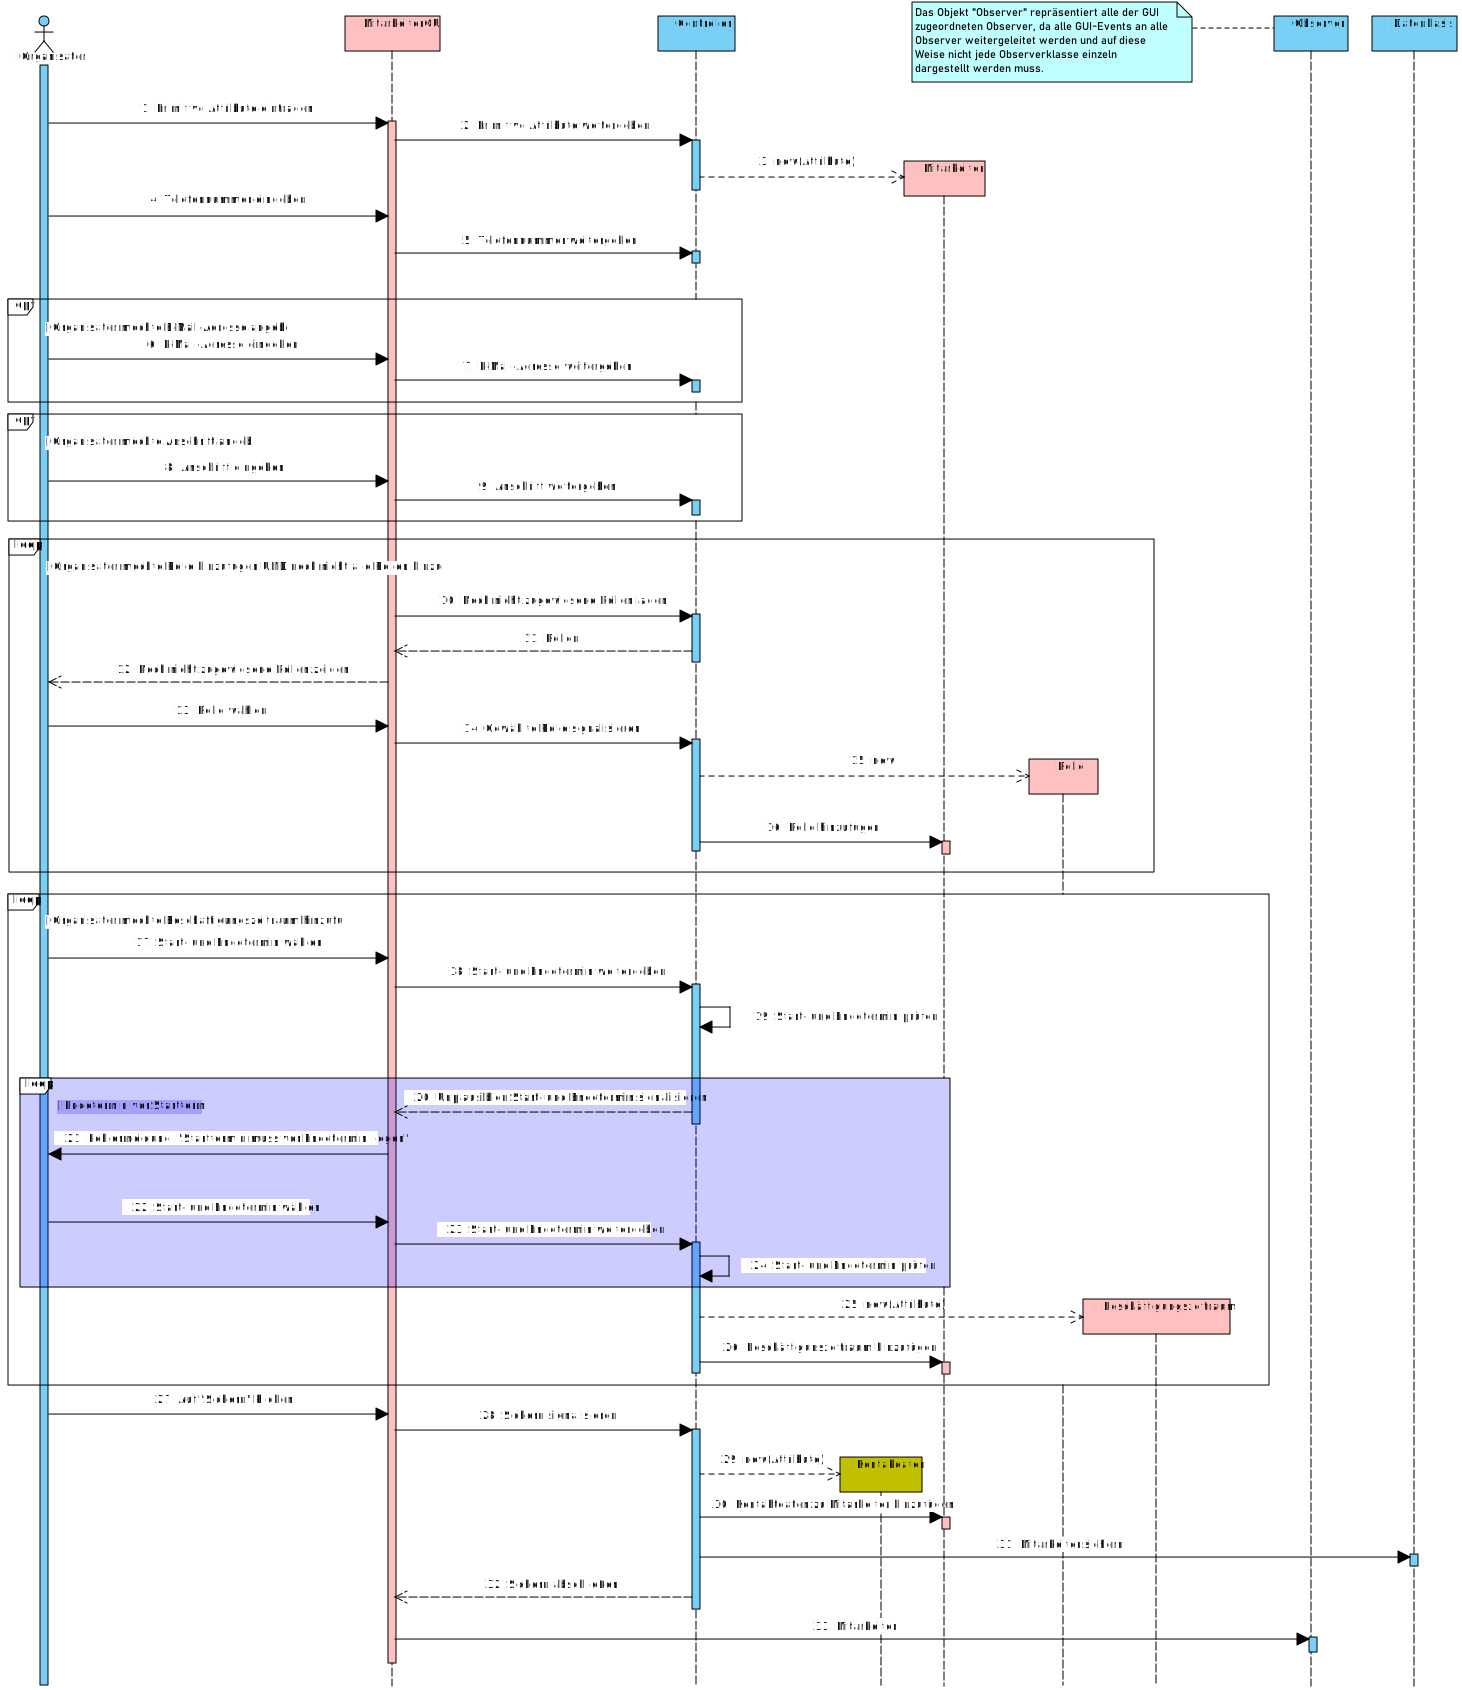
\includegraphics[width=0.98\columnwidth]{Bilder/seq_Mitarbeiter_anlegen.pdf}
    \caption{Szenario Mitarbeiter anlegen}
    \label{seq:mitarbeiter-anlegen}
\end{figure}

Das Anlegen eines Mitarbeiters wurde in \autoref{seq:mitarbeiter-anlegen} modelliert. Hier trägt der Organisator zunächst die primitiven Attribute des Mitarbeiters ein, aus denen dann ein Mitarbeiterobjekt erzeugt wird. Dann werden dessen Kontaktdaten hinterlegt. Hierzu wird ebenso vorgegangen wie in \autoref{seq:ansprechperson-anlegen} und dann das erstellte Kontaktdatenobjekt dem Mitarbeiterobjekt hinzugefügt. Als nächstes werden dem Mitarbeiter Rollen hinzugefügt. Dazu werden die dem Mitarbeiter noch nicht zugewiesenen Rollen angezeigt und der Organisator wählt die gewünschte Rolle aus. Basierend auf der Auswahl des Organisators wird ein neues Rollenobjekt erzeugt und dem Mitarbeiterobjekt hinzugefügt. Dieser Vorgang wird solange wiederholt, bis der Organisator dem Mitarbeiter keine Rollen mehr hinzufügen möchte oder er dem Mitarbeiter alle verfügbaren Rollen zugewiesen hat. Darum befindet sich dieser Vorgang in einem loop-Fragment. Als letztes werden dem Mitarbeiter Beschäftigungszeiträume zugewiesen. Auch derer kann ein Mitarbeiter beliebig viele besitzen, sodass auch die nachfolgenden Schritte Teil eines loop-Fragmentes sind. Der Organisator wählt zunächst Start- und Endetermin des Beschäftigungszeitraumes. Liegt der Starttermin vor dem Endetermin, wird eine Fehlermeldung angezeigt und der Organisator wird aufgefordert einen neuen Start- und Endetermin anzugeben. Dies wiederholt sich solange, bis der Starttermin vor dem Endetemin liegt, weshalb es sich auch hier um ein loop-Fragment handelt. Als nächstes wird aus den eben gewählten Attributen ein Beschäftigungszeitraumobjekt erzeugt und dieses dem Mitarbeiter hinzugefügt. Als letztes wird das Mitarbeiterobjekt gesichert und auf der Datenbasis gespeichert.

\FloatBarrier

\subsection{Hilfsmittel anlegen}

\begin{figure}[ht!]
    \centering
    \includegraphics[width=0.98\columnwidth]{Bilder/seq_Hilfsmittel_anlegen.pdf}
    \caption{Szenario Hilfsmittel anlegen}
    \label{seq:hilfsmittel-anlegen}
\end{figure}

Wie man in \autoref{seq:hilfsmittel-anlegen} erkennen kann, trägt der Organisator beim anlegen eines Hilfsmittels zunächst die primitiven Attribute des Hilfsmittels ein. Nun gibt es zwei in einem alt-Fragment dargestellte Pfade: Handelt es sich bei dem anzulegenden Hilfsmittel um ein Gebrauchsgut, so gibt der Organisator zunächst die Gesamtzahl an. Dann wird ein neues Gebrauchsgutobjekt erzeugt, welches zu einem Hilfsmittelobjekt gecastet wird. Handelt es sich um ein Verbrauchsgut, so gibt der Organisator die aktuelle Menge ein, sodass ein Verbrauchsgutobjekt erzeugt werden kann. Nun wird mittels einer Interaktionsreferenz das Sequenzdiagramm \enquote{Verweis anlegen} aufgerufen. Der entstandene Verweis wird dann dem Verbrauchsgutobjekt als Lieferant hinzugefügt und das Verbrauchsgutobjekt zu einem Hilfsmittelobjekt gecastet. Zuletzt hat der Organisator die Möglichkeit dem Hilfsmittel Bilder hinzuzufügen. Hierzu wird innerhalb eines loop-Fragments zunächst das Sequenzdiagramm \enquote{Bild anlegen} aufgerufen und das angelegte Bild dann dem Hilfsmittelobjekt hinzugefügt. Abschließend wird das Hilfsmittel gesichert und auf die Datenbasis geschrieben. 
